\section{Question 1: Vision \& Localization}

The first part of this question was to create a program capable of finding red blobs. The code would take an image captured by the webcam. It was then run through a series of filters. The first filter was a Gaussian filter that would blur the image. The next filters the image based on hue, and intensity of the image removing any non-red objects. Next the filtered image runs through another Gaussian filter. The final two filters are dilate and erode. The former caused the image to stretch while the latter decreases the resolution. This creates a white mask designates where red blobs are found. Next we determine the largest red blob as the blob we are looking for based on the assumption that all other red blobs are minor background noise.

We trained a Support Vector Machine with a Linear Kernel with the pixel coordinates as input data and motor values as labels. After training we then combined the sensor values from the camera with our predicted values from our motion model using a kalman filter. Between the predict and update stages of the kalman filter algorithm, we move the motors. An added while loop waits for the vision data.

\begin{verbatim}
# predict 
X, S = kf_predict(X, S, d*U)
# move
m_1.turn( d*20,120,False)
m_2.turn(-20,120,False)
z = None
while z == None:
		z = v.get_local()
Z = clf.predict(z)
# update
X, S = kf_update(X, S, Z)
\end{verbatim}

\begin{figure}[tbd]
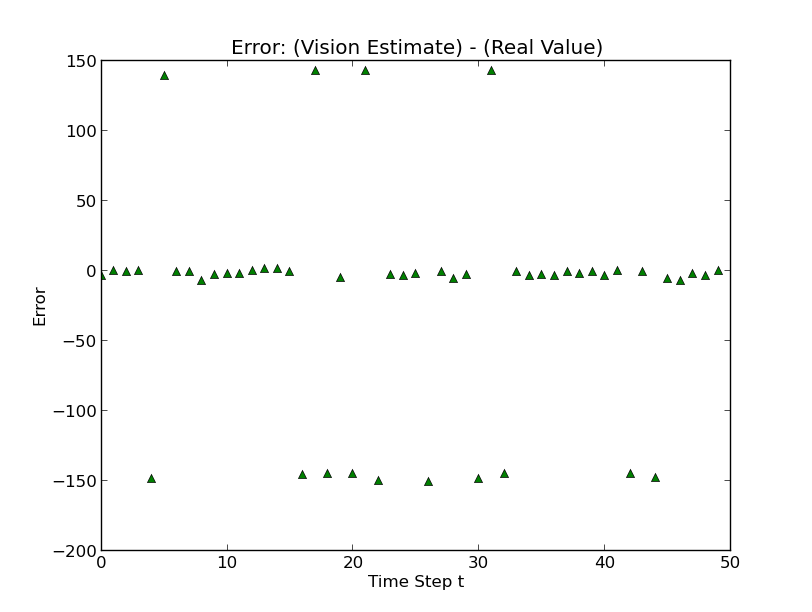
\includegraphics[width=0.5\textwidth]{images/vision_vs_real.png}
\caption{\label{vision_vs_real} Vision vs. Real}
\end{figure}

\begin{figure}[tbd]
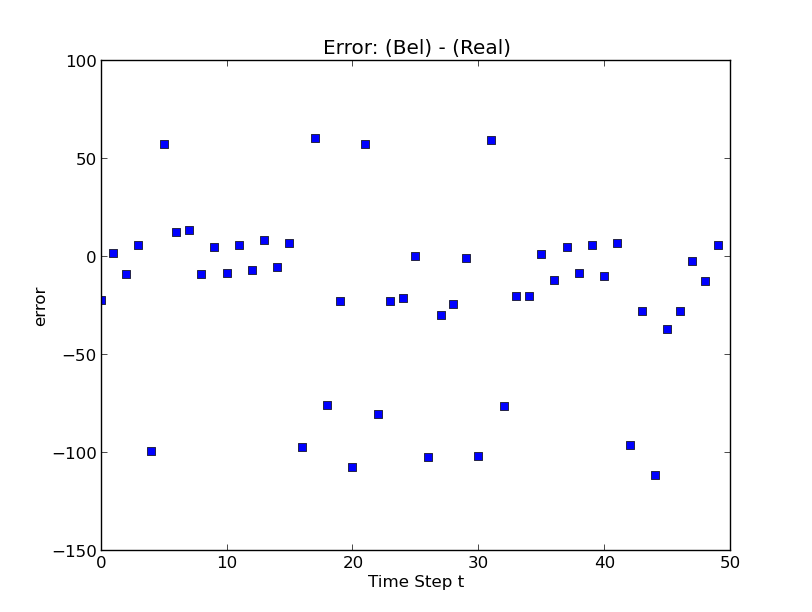
\includegraphics[width=0.5\textwidth]{images/bel_vs_real.png}
\caption{\label{bel_vs_real} Difference in Bel(x) and Real}
\end{figure}

\begin{figure}[tbd]
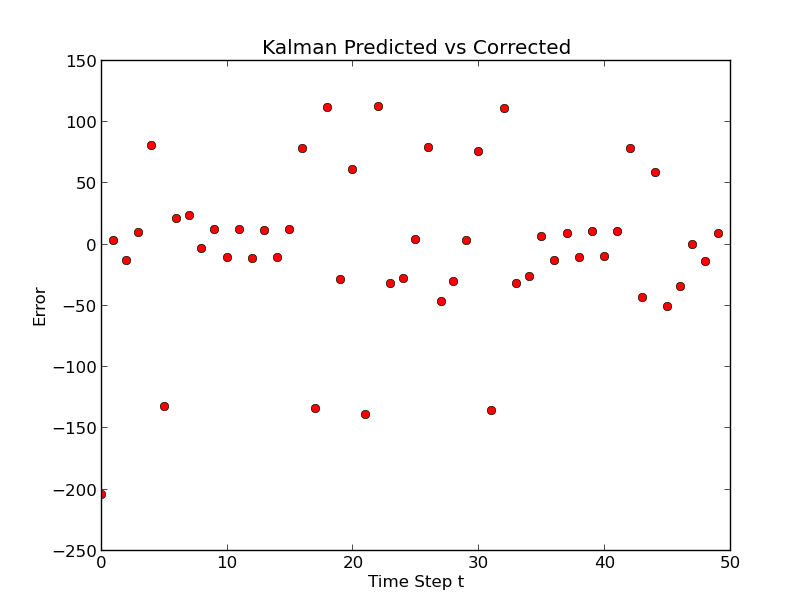
\includegraphics[width=0.5\textwidth]{images/pre_vs_cor.png}
\caption{\label{pre_vs_cor} Difference in Bel(x) between Predict and Update}
\end{figure}

\begin{figure}[tbd]
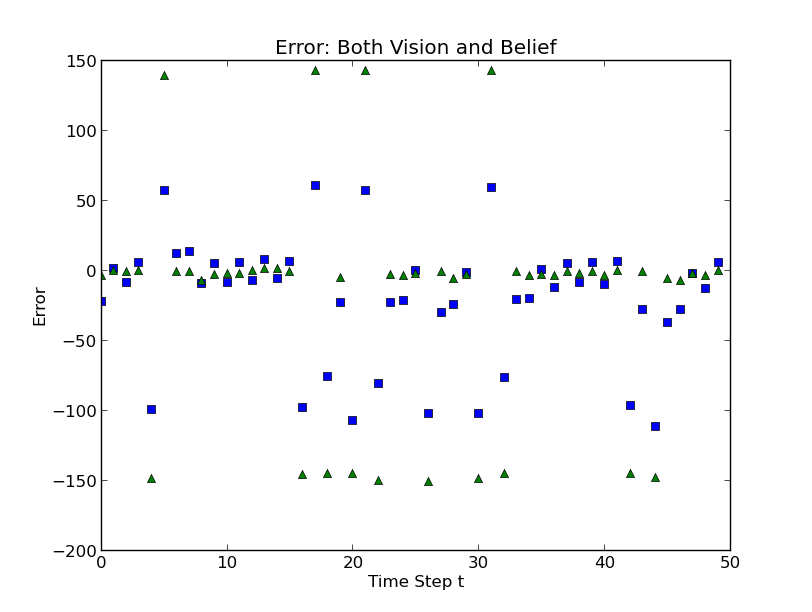
\includegraphics[width=0.5\textwidth]{images/both_vision_belief.png}
\caption{\label{both_vision_belief} Error in belief (Blue) and vision (Green)}
\end{figure}


